\scanpage{39}
\mspage{(20)}
repère \inserted{les} $u(\widetilde a_i^\omega)$, résulte déjà de celle de $\xi$, qui repère \inserted{les} $u(d_i^\omega)$,
\figure{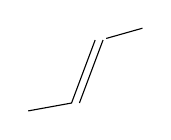
\begin{tikzpicture}[baseline=0pt]
\draw (0,0)--(.55,.10)--(.85,.90);
\draw (.65,.10)--(.95,.90);
\draw (.99,.92)--(1.45,1.05);
\end{tikzpicture}}
Les graphes $\overline{\underline{\mathrm{I}}}$ \unsure{à|:} $\overline{\underline{\mathrm{VII}}}$ donnent lieu au diagramme d'inclusions
\diagram{\begin{tikzcd}[ampersand replacement=\&,column sep=2em,row sep=2.8em,execute at end picture={
\coordinate (frameNW) at ([xshift=-4mm,yshift=5mm]\tikzcdmatrixname-2-1.north west);
\coordinate (frameSE) at ([xshift=5mm,yshift=-4mm]\tikzcdmatrixname-3-3.south east);
\coordinate (frameNE) at (frameNW -| frameSE);
\coordinate (frameSW) at (frameNW |- frameSE);
\draw ([xshift=2mm]frameNW)--([xshift=-2mm]frameNE);
\draw ([yshift=-3mm]frameNW)..controls ([yshift=-10mm]frameNW) and ([xshift=1mm,yshift=5mm]frameSW)..([xshift=1mm,yshift=2mm]frameSW);
\draw ([xshift=2mm]frameSW)--([xshift=-1mm]frameSE);
\draw ([yshift=-1mm]frameNE)--([yshift=-3mm]frameNE);
\draw ([yshift=-6mm]frameNE)--([yshift=1mm]frameSE);
\node[left=7mm] at (\tikzcdmatrixname-2-1.west) {$(68)$};
}]
\&\&\overline{\underline{\mathrm{III}}}\arrow[dl,hook']\arrow[dr,hook]\&\&\\
\overline{\underline{\mathrm{I}}}\arrow[r,hook]\arrow[dr,hook]\&\overline{\underline{\mathrm{II}}}\arrow[dr,hook]\arrow[r,phantom,"\unsure{\deleted{\leftrightarrow}|\leftrightarrow}" description]\&\phantom{\overline{\underline{\mathrm{II}}}}\&\overline{\underline{\mathrm{IV}}}\arrow[dl,hook']\&\mathrm{V}\arrow[l,hook']\\
\&\overline{\underline{\mathrm{VII}}}\arrow[r,hook]\&\overline{\underline{\mathrm{VI}}}\&\&
\end{tikzcd}}

Sans calcul, je peux déjà prédire que la donnée d'un autom. de $\overline{\underline{\mathrm{VII}}}$ fixant les sommets et commutant à $G_J$, équivaut à la donnée des quantités
\[
(69)\qquad (\uline{\lambda},\beta',\uline{\xi'})\in\widehat\Pi_{03}\times\widehat\Pi_{03}\times\widehat\Pi_{03}
\]
\margin{\(\underbrace{\begin{gathered}\text{donc }\beta'\\\text{inutile!}\end{gathered}}\)}
reliés par l\deleted{\unsure{es}}' équations \deleted{(63) ici}
\[
(70)\qquad\left\{\begin{aligned}
\beta'&=\alpha'\sigma_\infty(\lambda)\\
\beta'\sigma_\infty(\beta')&=1
\end{aligned}\right.\qquad
\begin{gathered}
\text{où}\quad\alpha'=\xi'\unsure{\rho^{\deleted{-1}}|\rho^{-1}}(\xi')^{-1}\\
\text{i.e.}\quad\alpha'\sigma_\infty(\lambda)\sigma_\infty(\alpha')\lambda=1
\end{gathered}
\]
(\unsure{tout} comme \inserted{dans le cas} $\overline{\underline{\mathrm{II}}}$ \inserted{$u$} est défini par \deleted{$(\lambda,\eta,\alpha')$},
\deleted{reliés par}
\[
(\unsure{69'})\qquad(\uline{\lambda},\uline{\eta},\alpha')\in\widehat\Pi_{0\unsure{,|.}3}\times\widehat\Pi_{03}\times\widehat\Pi_{03}
\]
avec l' équations
\margin{\begin{tabular}{@{}c@{}}donc $\alpha'$\\inutile!\end{tabular}}
\[
(70')\qquad\left\{\begin{aligned}
\beta'&=\alpha'\sigma_\infty(\lambda)\\
\alpha'\rho(\alpha')\rho^2(\alpha')&=1
\end{aligned}\right.\qquad\text{où}\quad\beta'=\eta\sigma_\infty(\eta)^{-1}
\]
\margin{38}
